\newchapter{Data Preparation}{ch:data-preparation}

One of the most important parts of any data science pipeline is data preparation. If the acquired data is not prepared in the right way, no matter how good the models are, optimal performance will be unattainable. Therefore, in this section, we are going to present all the steps we took to prepare our data for training. 

\section{Feature selection}

Samples in the IRMAS dataset consisted of three features, alongside the raw audio itself - length of the raw audio, the genre the song from the audio belongs to, and a Boolean value indicating the presence or absence of drums. However, due to the fact that these values only appear in the train set, and not in the given evaluation set, and without a way to extract them, we decided not to use features genre and drums, leaving us only with raw audio as the base feature. 

However, upon researching previous works in instrument and audio classification, we knew that models working with raw audio probably will probably not achieve the best results. As a result, we extracted a number of different features from the available raw audio and used those features as inputs to our models. Exact definitions of all the listed features have already been explained in the previous section, so this section will only focus on the exact way these features were extracted from raw audio and used in our models. Librosa \footnoteurlwithoutheader{https://librosa.org/} \space \space library was used to extract each of these features.

\subsection{MFCC}
\label{sec:data-prep:mfcc}

The first features we decided to try using were Mel-frequency cepstral coefficients (MFCC). The choice of using this feature was motivated by a couple of previous works achieving good results using MFCC, such as \cite{Racharla_2020} or \cite{Diment2013ModifiedGD}. MFCC features were calculated using the default Librosa's get\textunderscore mfcc method with the following parameters: the length of the Fast-Fourier transform (FFT) window was set to 2048, hop length was 512, and the sampling rate was usually set to the default sampling rate of our audio, 44100 Hz. We choose 40 as the number of MFC coefficients, which is a bit higher than the usual number (13). We chose a higher value as we believed the model we used had enough capacity to be able to fully benefit from the additional information provided by using more coefficients. The output of the method was a 2D feature matrix which was resized to the dimensions 256x40, simply to standardize the dimensions of inputs to our model.

\subsection{Mel spectrograms}

The second type of features extracted from audio we decided on using were mel-spectrograms (further referred to as just spectrograms), as they were by far the most prevalent features used in most previous work we analyzed and seemed to be the most promising ones. They also enabled us to treat the problem of instrument detection as a computer vision problem, instead of an audio one, as a generated spectrogram is nothing more but an image. This allowed us to approach the problem from another angle, as well as to use a larger spectre of models and algorithms. When generating spectrograms, the following values were used:
number of mel bands was set to 256, yet again in hopes that a higher value will allow our models to extract more information from the input audio. FFT window was set to 2048 and hop length to 512 (25\% of the length of the FFT window). The sampling rate was set to the default sampling rate of input audio, 44100 Hz. The resulting image was resized to 256x256 pixels to standardize the dimensions of spectrograms entering the model. As the resulting spectrogram was a single-channel image, the values of the channel were repeated 3 times in order to acquire a 3-channel image which our model expected.

\subsection{General audio features}

Finally, we decided to try and combine multiple audio features into a single matrix which would then be provided as input to our models. We assumed that by combining multiple features our model would be able to extract more information about the input audio and thus work better than with only one of the features. The features we selected for combining were, as follows:

\begin{itemize}
    \item MFCC
    \item Chroma features
    \item Zero-crossing rate
    \item Spectral centroid 
    \item Root-Mean-Square-Energy
    \item Spectral contrast
    \item Spectral bandwith
    \item Spectral roll-off
    \item Spectral flatness
    \item Polynomial features
\end{itemize}

Tonnetz features were also the ones we initially considered, but finally decided not to use, as our ANOVA in Section~\ref{sec:statistical-testing} showed that its mean values do not significantly differ across different (instrument) groups. Each feature was created using the default values from the corresponding Librosa method. This meant that in this instance we used 13 for the number of Mel coefficients when generating MFCC, as it is the default value. In this case, we felt that we already increased the amount of information by a large margin by incorporating all the other features, so there was no need for the extra information gained by using 40 as the number of Mel coefficients when generating MFCC. Every feature was generated as a matrix of dimensions {$M_{n_i} \times N$}, where {$n_i$} represents the number of rows for the $i$-th feature, and $N$ depends on the length of the input audio. All of the features were then combined into a single matrix of dimensions $40 \times N$ , whose rows (40) were then passed into the model as separate channels. This approach of combining multiple features into a single vector is similar to the one used in \cite{Racharla_2020}, although we use more features in our approach and take the entire MFCC feature matrix as input, whereas authors from \cite{Racharla_2020} calculate the mean of each Mel coefficient column to create the final input, resulting in a $1 \times 13$ vector, compared to our $259 \times N$ matrix.

\section{Collecting new data -- Audioset}
\label{sec:data-prep:collecting-audioset}

As already described in section 4, due to quality concerns with the IRMAS dataset, and in an attempt to acquire more data, we downloaded a subset of the Audioset dataset containing only examples from target classes. We've used Google's original files \texttt{class\_labels\_indices.csv}, \texttt{balanced\_train\_segments.csv}, and \texttt{unbalanced\_train\_segments.csv}\footnoteurl{https://research.google.com/audioset/index.html}{https://research.google.com/audioset/index.html}. The file \\ \texttt{balanced\_train\_segments.csv} contains mappings from their string unique IDs to actually recognizable classes, such as the mapping from \texttt{/m/01xqw} to "Cello". The files \texttt{balanced\_train\_segments.csv} and \texttt{unbalanced\_train\_segments.csv} both contain columns YTID, start\_seconds, end\_seconds, and positive\_labels. The only difference is that, as the names suggest, the labels are balanced in one file, and unbalanced in the other. A small example of actual values from \texttt{balanced\_train\_segments.csv} is shown in Table~\ref{tab:balanced-train-segments}. YTID is the unique YouTube identifier that needs to be appended to \texttt{"https://www.youtube.com/watch?v="}. Columns start\_seconds and end\_seconds suggest the start and end time of a 10 second window. These columns were used to crop the audio after downloading it. We downloaded just the audio from the video. Unfortunately, we did not find a library with the option of downloading a YouTube video (audio) with the given time range. Instead, after downloading the video using the pytube\footnoteurl{https://pytube.io/en/latest/}{https://pytube.io/en/latest/} library, ffmpeg\footnoteurl{https://github.com/kkroening/ffmpeg-python}{https://github.com/kkroening/ffmpeg-python} library for Python was used to crop the audio and save it to the .mp3 format. This saving to the .mp3 format turned out to be a mistake, as librosa, which uses libsndfile\footnoteurl{https://github.com/libsndfile/libsndfile}{https://github.com/libsndfile/libsndfile} in the background, does not support .mp3 files, and switches to using audioread\footnoteurl{https://github.com/beetbox/audioread}{https://github.com/beetbox/audioread} instead, which takes much longer. Thus, all the file were converted to the vaw format first using a single channel, $44.1$ kHz sample rate, and \texttt{pcm\_s16le} audio\ codec.

\begin{table}[H]
\centering
\begin{tabular}{c c c c}
\hline
YTID & start\_seconds & end\_seconds & positive\_labels \\ \hline
$--$PJHxphWEs & 30.000 & 40.000 & \texttt{"/m/09x0r,/t/dd00088"} \\
$--$ZhevVpy1s & 50.000 & 60.000 & \texttt{"/m/012xff"} \\
$--$aE2O5G5WE & 0.000 & 10.000 & \texttt{"/m/03fwl,/m/04rlf,/m/09x0r"} \\
$--$aO5cdqSAg & 30.000 & 40.000 & \texttt{"/t/dd00003,/t/dd00005"}
\end{tabular}
\caption{A small sample from the \texttt{balanced\_train\_segments.csv} file}
\label{tab:balanced-train-segments}
\end{table}

When downloading the dataset, we occurred numerous VideoNotAvailable warnings, due to the videos being made private or removed. Surprisingly, we did not occur any blacklisting from YouTube due to a large number of GET request in a short period of time. We did, however, notice problems from our service providers. Namely, as soon as we would lose the connection to the internet (for whatever reason), pytube would throw a large number of URLError class exceptions. This is because it would continue looping over the YTIDs, trying to fetch them, but would fail so (because of the loss of connection) and would interpret it as the URLError. This proved to be a problem even for short-timed disconnections, such as few seconds, because a computer can loop over many examples in a second. At first, we thought that this is the short-time blacklisting from YouTube side. However, it was not. Finally, we solved this problem by setting up a try-except block and sleeping for 60 seconds whenever catching a URLError class exception, which happened rarely, but caused skipping a large number of YTIDs.

\begin{table}[H]
\centering
\begin{tabular}{l l l}
\hline
Audioset ID & Description & Class \\ \hline
"/m/02qldy" & narration & \texttt{voi} \\
"/m/01h8n0" & conversation & \texttt{voi} \\
"/m/02zsn" & female speech & \texttt{voi} \\
"/m/05zppz" & male speech & \texttt{voi} \\
"/t/dd00005" & child singing & \texttt{voi} \\
"/t/dd00004" & female singing & \texttt{voi} \\
"/t/dd00003" & male singing & \texttt{voi} \\
"/m/0l14jd" & choir & \texttt{voi} \\
"/m/07y\_7" w/o "/m/0d8\_n" & violin, fiddle w/o pizzicato & \texttt{vio} \\
"/m/07gql" & trumpet & \texttt{tru} \\
"/m/06ncr" & saxophone & \texttt{sax} \\
"/m/05r5c" w/o "/m/01s0ps" & piano w/o electric piano & \texttt{pia} \\
"/m/013y1f" & organ (hammond and electronic) & \texttt{org} \\
"/m/02sgy" & electric guitar & \texttt{gel} \\
"/m/042v\_gx" & acoustic guitar & \texttt{gac} \\
"/m/0l14j\_" & flute & \texttt{flu} \\
"/m/01wy6" & clarinet & \texttt{cla} \\
"/m/01xqw" & cello & \texttt{cel}
\end{tabular}
\caption{Audioset IDs of interest}
\label{tab:audioset-ids}
\end{table}

Before downloading the YouTube audio, we first checked if any of the positive labels we were interested in was contained within the positive\_labels column. In Table~\ref{tab:audioset-ids} we show all the IDs we were interested in, along with some we were trying to avoid (pizzicato and electric piano). Some categories, such as "guitar", were general, and contained sub-categories, such as electric, bass, acoustic, steel guitar etc. That called for additional checks so that no unwanted categories get included. Checkpointing to a csv file was done every few thousand iterations, so that no progress is lost in case of exceptions. Although there were sometimes multiple \texttt{voi} class sources possible, we made sure to label \texttt{voi} as positive only once. 

Finally, although all the files were said to have a duration of 10 seconds, we found that not to be the case. Consequently, we removed the files which were either shorter or longer than 10 seconds by more than 0.5 seconds. For all the other files, we padded them with zeros or truncated them. This removed around $0.1$ \% of the files. A bit larger number of files were padded, but the padding was usually much lower than 0.5 seconds. The new mean and standard deviation values were calculated for performing normalization on Audioset.

\section{Normalization}

Normalizing input data is a common technique in deep learning, usually done to help with the convergence of the gradient descent algorithm. There are a couple of different ways normalization could be done -- we decided on normalizing audio input to have a mean of 0 and standard deviation of 1. In order to do so, we calculated the mean and standard deviation of audio files (loaded as Numpy arrays) on the train set, and then used those values when normalizing the input values according to the formula:

\[ \text{{New value}} = \frac{{\text{{value}} - \text{{mean}}}}{{\text{{standard deviation}}}} \]

Only audio files were normalized, meaning that spectrograms or MFCC features generated from those audio files were not additionally normalized, with the exception of spectrograms passed to the Audio Spectrogram Transformer.

\section{Augmentations}

Due to the relatively small number of examples in the IRMAS dataset, and in an attempt to improve the generalization capabilities of our models, we decided to implement multiple augmentation strategies. The augmentation strategies can be split into two groups: augmentations done on the raw audio, and augmentations done on spectrograms. In all cases, all possible augmentations for the given features were used, meaning that, for example, if we were using spectrograms as inputs to our models, we would first augment the original audio files using audio augmentations, then additionally augment the spectrograms generated from those audio files. On the other hand, if we were using raw audio or general audio features, then only augmentations on raw audio would be used. 


\subsection{Audio augmentations}

\subsubsection{Noise injection}

This is a common type of audio augmentation, often used in different types of audio-related machine learning. It consists of generating a noise sample from a distribution (i.e. Gaussian distribution), multiplying it by a small number, and adding it to the original audio. Simply, we can write:


\[ \text{{Augmented audio}} = \text{{Original audio}} + \alpha \times \text{{Noise}} \]

Where $\alpha$ represents a small number used to make sure the added noise does not overpower the original signal.

In our experiments, we used noise generated from a Gaussian distribution \textbf{with the mean and standard deviation equal to the mean and standard deviation of the training dataset}. An example of applying the augmentation can be seen in Figure~\ref{fig:noise-injection}

\begin{figure}[H]
        \centering
        
        \begin{minipage}{0.49\textwidth}
            \centering
            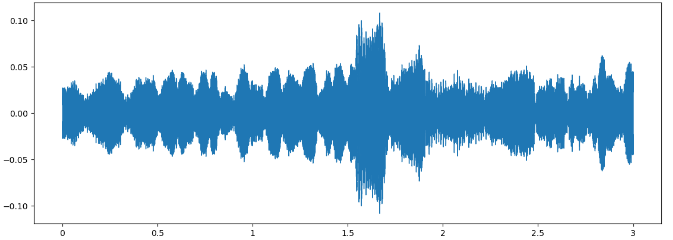
\includegraphics[width=\linewidth]{images/noise_augmentation_original_signal_intensity.png}
            \caption*{Original signal}
        \end{minipage}%
        \hfill%
        \begin{minipage}{0.49\textwidth}
            \centering
            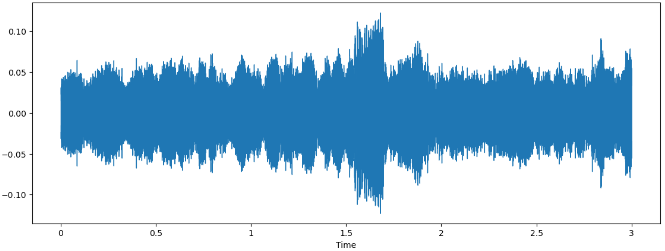
\includegraphics[width=\linewidth]{images/noise_augmentation_augmented_signal_01_intensity.png}
            \caption*{Original signal after noise injection}
        \end{minipage}
        
        \vspace{0.5cm}
        
        \begin{minipage}{0.49\textwidth}
            \centering
            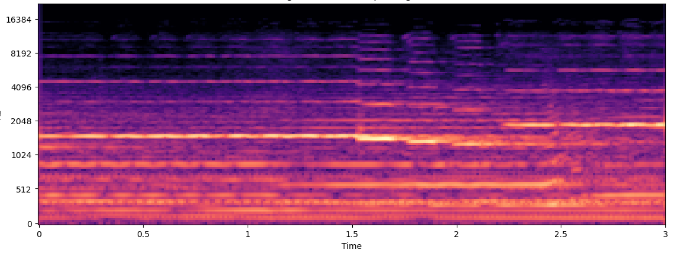
\includegraphics[width=\linewidth]{images/noise-injection-original-spectogram.png}
            \caption*{Mel-spectrogram of the original signal}
        \end{minipage}%
        \hfill%
        \begin{minipage}{0.49\textwidth}
            \centering
            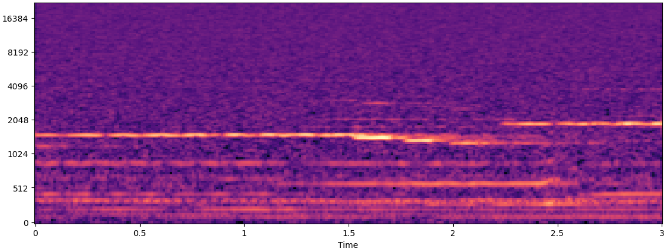
\includegraphics[width=\linewidth]{images/noise-injection-augmented-spectogram.png}
            \caption*{Mel-spectrogram of the signal after noise injection}
        \end{minipage}
                
        \centercaption{Example of the effect of noise injection, alpha=0.1}
        
        \label{fig:noise-injection}
        
    \end{figure}

Although the signal intensity plot does not show much difference between the original and augmented signal, the difference is obvious when looking at the mel-spectrogram representations of the signal. It also clarifies that using a too-large alpha value can significantly degrade the original signal, and depending on the representation used, potentially harm training. That is why we decided to choose a more conservative alpha value of 0.005 in our experiments.

\subsubsection{Pitch shift}

The second type of audio augmentation we used is pitch shift. This type of audio augmentation consists of shifting the pitch of the input signal by a random amount. In our experiments, we shifted the signal by a random number of semitones generated uniformly in range [-6,6]. It is important not to shift the pitch of the original signal too much, as it could end up outside the normal pitch range for that instrument. The effects of pitch shift augmentation can be seen in Figure~\ref{fig:pitch-shift}.

\begin{figure}[H]
        \centering
        
        \begin{minipage}{0.49\textwidth}
            \centering
            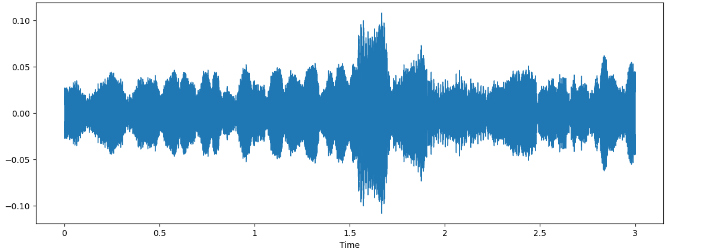
\includegraphics[width=\linewidth]{images/pitch-shift-original-audio-intensity.png}
            \caption*{Original signal}
        \end{minipage}%
        \hfill%
        \begin{minipage}{0.49\textwidth}
            \centering
            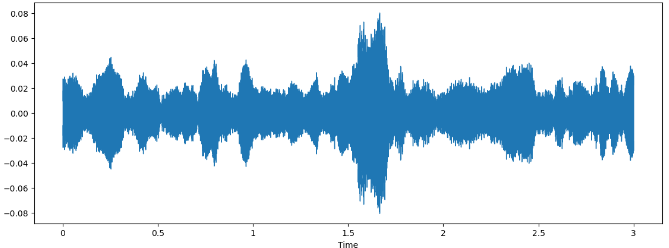
\includegraphics[width=\linewidth]{images/pitch-shift-augmented-audio-intensity.png}
            \caption*{Original signal after pitch shift}
        \end{minipage}
        
        \vspace{0.5cm}
        
        \begin{minipage}{0.49\textwidth}
            \centering
            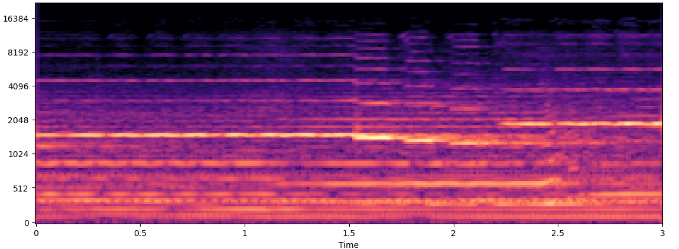
\includegraphics[width=\linewidth]{images/pitch-shift-original-audio-spectogram.png}
            \caption*{Mel-spectrogram of the original signal}
        \end{minipage}%
        \hfill%
        \begin{minipage}{0.49\textwidth}
            \centering
            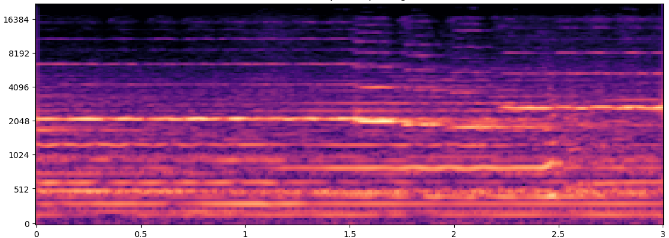
\includegraphics[width=\linewidth]{images/pitch-shift-augmented-audio-spectogram.png}
            \caption*{Mel-spectrogram of the signal after pitch shift}
        \end{minipage}
                
        \centercaption{Example of the effect of pitch shift up by 6 semitones}
        
        \label{fig:pitch-shift}
        
    \end{figure}

We can easily see the effects of the pitch shift in spectrograms in Figure~\ref{fig:pitch-shift}. We can see the yellow lines representing the presence of certain frequencies clearly shift up in the augmented spectrogram, compared to the original one.

\subsubsection{Time shift}

Finally, the third audio augmentation used is time shift. It consists of moving the entire signal by a certain amount forward or backward, so it starts and ends on a different part of the signal. The duration of the signal is not changed.  Let's say we time shift the original signal by 1 second forward. That would mean that the new signal now starts at the previous signal's one-second mark, and its last second is what used to be the first second of the original signal. The effect of this augmentation is best seen through visualizations in Figure~\ref{fig:time-shift}.

\begin{figure}[H]
        \centering
        
        \begin{minipage}{0.49\textwidth}
            \centering
            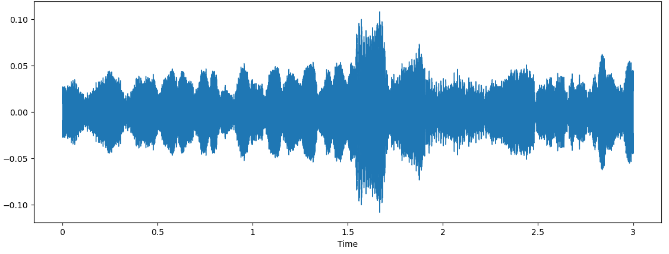
\includegraphics[width=\linewidth]{images/time-shift-original-intensity.png}
            \caption*{Original signal}
        \end{minipage}%
        \hfill%
        \begin{minipage}{0.49\textwidth}
            \centering
            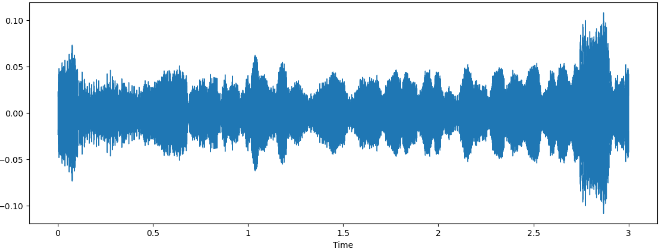
\includegraphics[width=\linewidth]{images/time-shift-augmented-intensity.png}
            \caption*{Original signal after time shift}
        \end{minipage}
        
        \vspace{0.5cm}
        
        \begin{minipage}{0.49\textwidth}
            \centering
            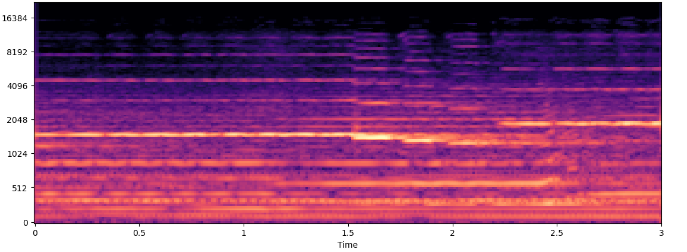
\includegraphics[width=\linewidth]{images/time-shift-original-spectogram.png}
            \caption*{Mel-spectrogram of the original signal}
        \end{minipage}%
        \hfill%
        \begin{minipage}{0.49\textwidth}
            \centering
            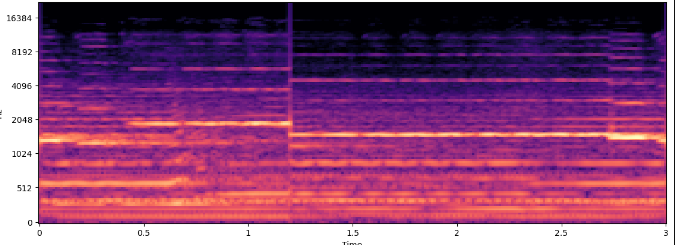
\includegraphics[width=\linewidth]{images/time-shift-augmented-spectogram.png}
            \caption*{Mel-spectrogram of the signal after time shift}
        \end{minipage}
                
        \centercaption{Example of the effect of time shift up 40\% of original length forwards}
        
        \label{fig:time-shift}
        
    \end{figure}

In our experiments, we performed time shifting by first randomly choosing a percentage in range [-0.4, 0.4], and then performing time shifting by shifting the original signal by the percentage of its original length forwards (if the chosen number was positive), or backward (if the chosen number was negative).

\subsection{Spectrogram augmentations}

The two spectrogram augmentations used in our experiments, time and frequency masking, were first introduced in \cite{specaugment}. The authors justify these augmentations by saying "These features (mel-spectrograms) should be robust to deformations in the time direction, partial loss of frequency information, and partial loss of small segments of speech." The essential idea of both techniques is the same - mask a part of the input spectrogram, forcing the model not to rely too much on any specific feature or part of the spectrogram, instead encouraging it to learn from more features, thus increasing its generalization.

\subsubsection{Frequency masking}

The first of these augmentations is frequency masking. As its name suggests, it consists of masking a block of consecutive mel frequency channels in the original mel spectrogram. The mask itself simply consists of the mean values of the entire spectrogram; this is important so as to not introduce any "foreign" information into the spectrogram. More formally, frequency masking is applied so that \textit{f} consecutive mel frequency channels $[f_0, f_0 + f)$ are masked, f being chosen uniformly in range [0, F], F being the frequency mask parameter, while $f_0$ is chosen in range $[0, v - f)$, where $v$ is the number of mel frequency channels. The effects of frequency masking can be seen in Figure~\ref{fig:frequency-masking}

\asideimages{7cm}{7cm}
	    {frequency-masking-original}
	    {Original spectrogram}
        {frequency-masking-augmented}
	    {Spectrogram after frequency masking}
	    {Example of the effect of frequency masking augmentation using two frequency masks}
	    {fig:frequency-masking}

During our experiments, we consistently created two frequency masks, with each mask occupying a portion (P) of the total frequencies. The value of P was uniformly selected from [0,10]. As two masks were used, the percentage of total frequencies masked in any given spectrogram could be at most 20\% and on average 10\%.

\subsubsection{Time masking}

The second type of spectrogram augmentation is time masking. It is, in essence, equivalent to frequency masking, except that it is done in the time domain of the spectrogram. Formally, time masking is applied so that $t$ consecutive time steps $[t_0, t_0 + t)$ are masked, where t is uniformly chosen in range $[0, T]$, $T$ being the time mask parameter, and $t_0$ chosen uniformly from $[0, \tau - t)$. $\tau$ is the number of time steps in the mel spectrogram. The effects of time masking can be seen in Figure~\ref{fig:time-masking}.

\asideimages{7cm}{7cm}
	    {frequency-masking-original}
	    {Original spectrogram}
        {time-masking-augmented}
	    {Spectrogram after time masking}
	    {Example of the effect of time masking augmentation using two time masks}
	    {fig:time-masking}

Same as in frequency masking, we always generated two time masks, each occupying P of the total time steps, P being chosen uniformly in range [0,10].

\subsubsection{Time + frequency masking}

Finally, we can see the combined effects of time and frequency masking in Figure~\ref{fig:time-frequency-masking}.

\asideimages{7cm}{7cm}
	    {frequency-masking-original}
	    {Original spectrogram}
        {time-frequency-masking-combined}
	    {Spectrogram after time and frequency masking}
	    {Example of the combined effect of time and frequency masking augmentation using two time and frequency masks}
	    {fig:time-frequency-masking}

\section{Dynamic sampling}
\label{sec:data-prep:dynamic-sampling}

The specific nature of the IRMAS dataset is, as has already been stated, that all the examples from the train set contain only a single label, while the examples in the test set may contain multiple labels per example. To mitigate this problem, instead of combining multiple train samples once and creating a single new set of training data with multiple labels,  we decided to implement a different approach we named \textbf{dynamic sampling}. In short, new training examples would be generated dynamically during training by randomly selecting and combining multiple examples with a single label into a new example containing multiple labels. In theory, this should greatly increase the variability of available data, as well as solve the issue of the training data having only a single label per example. In addition, it would save the space that static examples overlapping would occupy.

We implemented two types of dynamic sampling - true dynamic sampling, and base-sample-persistent dynamic sampling. We are going to shortly explain their differences and implementation, while the results we achieved will be presented in Chapter~\ref{ch:evaluation}.

\subsection{True dynamic sampling}

The "true" in the name of this type of dynamic sampling comes from the fact that every original example from which the final combined example consists is randomly selected at the moment the dynamic sampling function is called, thus meaning there is no dependency between two dynamic sampling calls or dependency between samples created in one epoch and another. The pseudocode for this sampling method is shown below:

\begin{algorithm}[H]
    \SetKwInOut{Input}{Input}
    \SetKwInOut{Output}{Output}

    \underline{function SampleTrueDynamic} $(minSampled, maxSampled, noClasses)$\;
    \Input{Minimum and maximum number of sampled examples, the total number of classes}
    \Output{sampled audio, list of labels in combined audio}
    noSamples = Random$(minSampled, maxSampled)$\;
    chosenLabels = RandomlySelectDistinctLabels$(noClasses, noSamples)$\;
    combinedAudio = None\;
    \For {label in chosenLabels}{
    \tcp{selects random audio out of all possible samples with the exception of samples with label \textit{label}} 
    audio = SelectRandomAudioExcludingLabel$(label)$ \;
    combinedAudio = CombineAudio$(combinedAudio, audio)$ \;
    }
    return combinedAudio, chosenLabels \;
    \caption{True dynamic sampling}
\end{algorithm}

Of course, this pseudocode only shows the sampling of a single sample; when training a model using dynamic sampling this method would be called many times, each time resulting in a new dynamically sampled example, made by combining multiple examples with single labels into a new example with multiple labels. Of course, a careful reader will have already asked themselves the following question: if the samples are now dynamically generated, how many samples should I generate, if I want to maximally utilize the data I already have available? And that is an excellent question, as due to the stochastic nature of the sampling process we have no guarantee of which original samples get sampled, possibly resulting in some examples being chosen for sampling many times, while other examples are not being chosen a single time. In order to solve this, you can use the following formula:

\DynamicSamplingNoSamples

The $N$ in the formula denotes the number of dynamic samples you have to generate to make sure that, on average, only $P$ \% of the total number of original examples do not get sampled within one epoch. $n$ is the total number of original examples, while minSampled and maxSampled represent the minimal and maximal number of original examples used when constructing a new, dynamically generated sample. The smaller the minSampled and maxSampled are, the larger $N$ has to be to maintain the same $P$. Table~\ref{tab:num-dynamic-samples} illustrates the effect  minSampled and maxSampled have on $N$, assuming $n$ is equal to the number of samples in the IRMAS training set, 6705, and $P$ value of 0.1\%, which we used in our experiments: 

\begin{table}[H]
\centering
\begin{tabular}{ccc}
\hline
minSampled & maxSampled & N     \\ \hline
1          & 2          & 30875 \\
1          & 3          & 23156 \\
1          & 4          & 18525 \\
1          & 5          & 15437
\end{tabular}
\caption{Effect of the minimal and maximal number of examples sampled using dynamic sampling on N}
\label{tab:num-dynamic-samples}
\end{table}

We can see that, if we want to dynamically sample and merge only two of the original samples at a time, we need to generate more than 30,000 dynamic samples, or almost 6x the size of the original dataset. On the other hand, if we dynamically sample and merge up to five original samples at a time, then a number of 15,437 suffices, which is rather more manageable. That is why in our experiments we usually used 4 or 5 for the value of maxSampled, while, of course, keeping minSampled at 1, as to sample certain examples as is.

One important advantage of this sampling method, in contrast, to sequentially iterating over examples in the training dataset, is that it follows a two-step process. Firstly, we uniformly choose the labels of the examples we intend to merge. Secondly, we uniformly select an example from all the available examples with each chosen label. Consequently, this approach ensures that, on average, every label (class) is sampled an equal percentage of times, thereby naturally balancing the distribution of classes within the dataset and increasing the macro performance metrics.


\subsection{Base-sample-persistent dynamic sampling}

The second type of dynamic sampling we considered is base-sample-persistent dynamic sampling. It is similar to true dynamic sampling, except for the following difference: the sampling method receives an initial sample (audio) and then builds upon it by selecting additional samples and merging them with the base sample. In practice, you would iterate over every sample \textbf{in the original training set}, assigning that sample the role of the base-sample, and, using base-sample-persistent dynamic sampling, merge it with $N$ other randomly chosen samples. This way, the base samples are consistent through every epoch; the only difference is the samples they are merged with.

The main idea behind this approach is to deal with very high variability in data which occurs when using true dynamic sampling, possibly leading to unstable training and the inability of the network to learn the distribution of samples. Furthermore, this sampling method \textbf{does not require} a large number of samples to work as does true dynamic sampling; as the base sample remains the same in every epoch, we have a guarantee that every sample from the original training data is going to get chosen at least once per epoch and usually more. The pseudocode of the algorithm is shown below: 

\begin{algorithm}[H]
    \SetKwInOut{Input}{Input}
    \SetKwInOut{Output}{Output}

    \underline{function SampleBasePersistent} $(baseSample, minSampled, maxSampled, noClasses)$\;
    \Input{Base sample, minimum and maximum number of sampled examples, the total number of classes}
    \Output{sampled audio, list of labels in combined audio}
    noSamples = Random$(minSampled, maxSampled)$\;
    chosenLabels = RandomlySelectDistinctLabels$(noClasses, noSamples)$\;
    \For {label in chosenLabels}{
    \tcp{selects random audio out of all possible samples with the exception of samples with label \textit{label}} 
    audio = SelectRandomAudioExcludingLabel$(label)$ \;
    baseSample = CombineAudio$(combinedAudio, baseSample)$ \;
    }
    return baseSample, chosenLabels \;
    \caption{Base-sample-persistent dynamic sampling}
\end{algorithm}

\section{Data splits}

We split the available datasets into training, validation, and testing datasets. The same splits were then used for training, validation, and testing of every model, to enable better comparison between models.

\subsection{IRMAS}
For IRMAS, we used the original train set in unchanged form as our train set. This dataset consisted only of examples with a single label. To generate validation and test sets, we split the provided evaluation dataset, which consisted of examples with one and more labels, into validation and test sets using a ratio of 70-30. After the split, the validation dataset consisted of 862 examples and the test dataset of 2010 examples. The training dataset remained unchanged at 6704 examples. 

\subsection{Audioset}

We collected a total number of 20,884 samples from the original Audioset dataset. Those samples were then split into training, validation, and testing datasets using a ratio of 70-10-20, resulting in the training set of size 14,618 examples, a validation set of size 2088, and a testing set of size 4176.